\documentclass{standalone}

\usepackage{tikz}
\usepackage{circuitikz}
\usepackage{pgfplots}
\begin{document}
	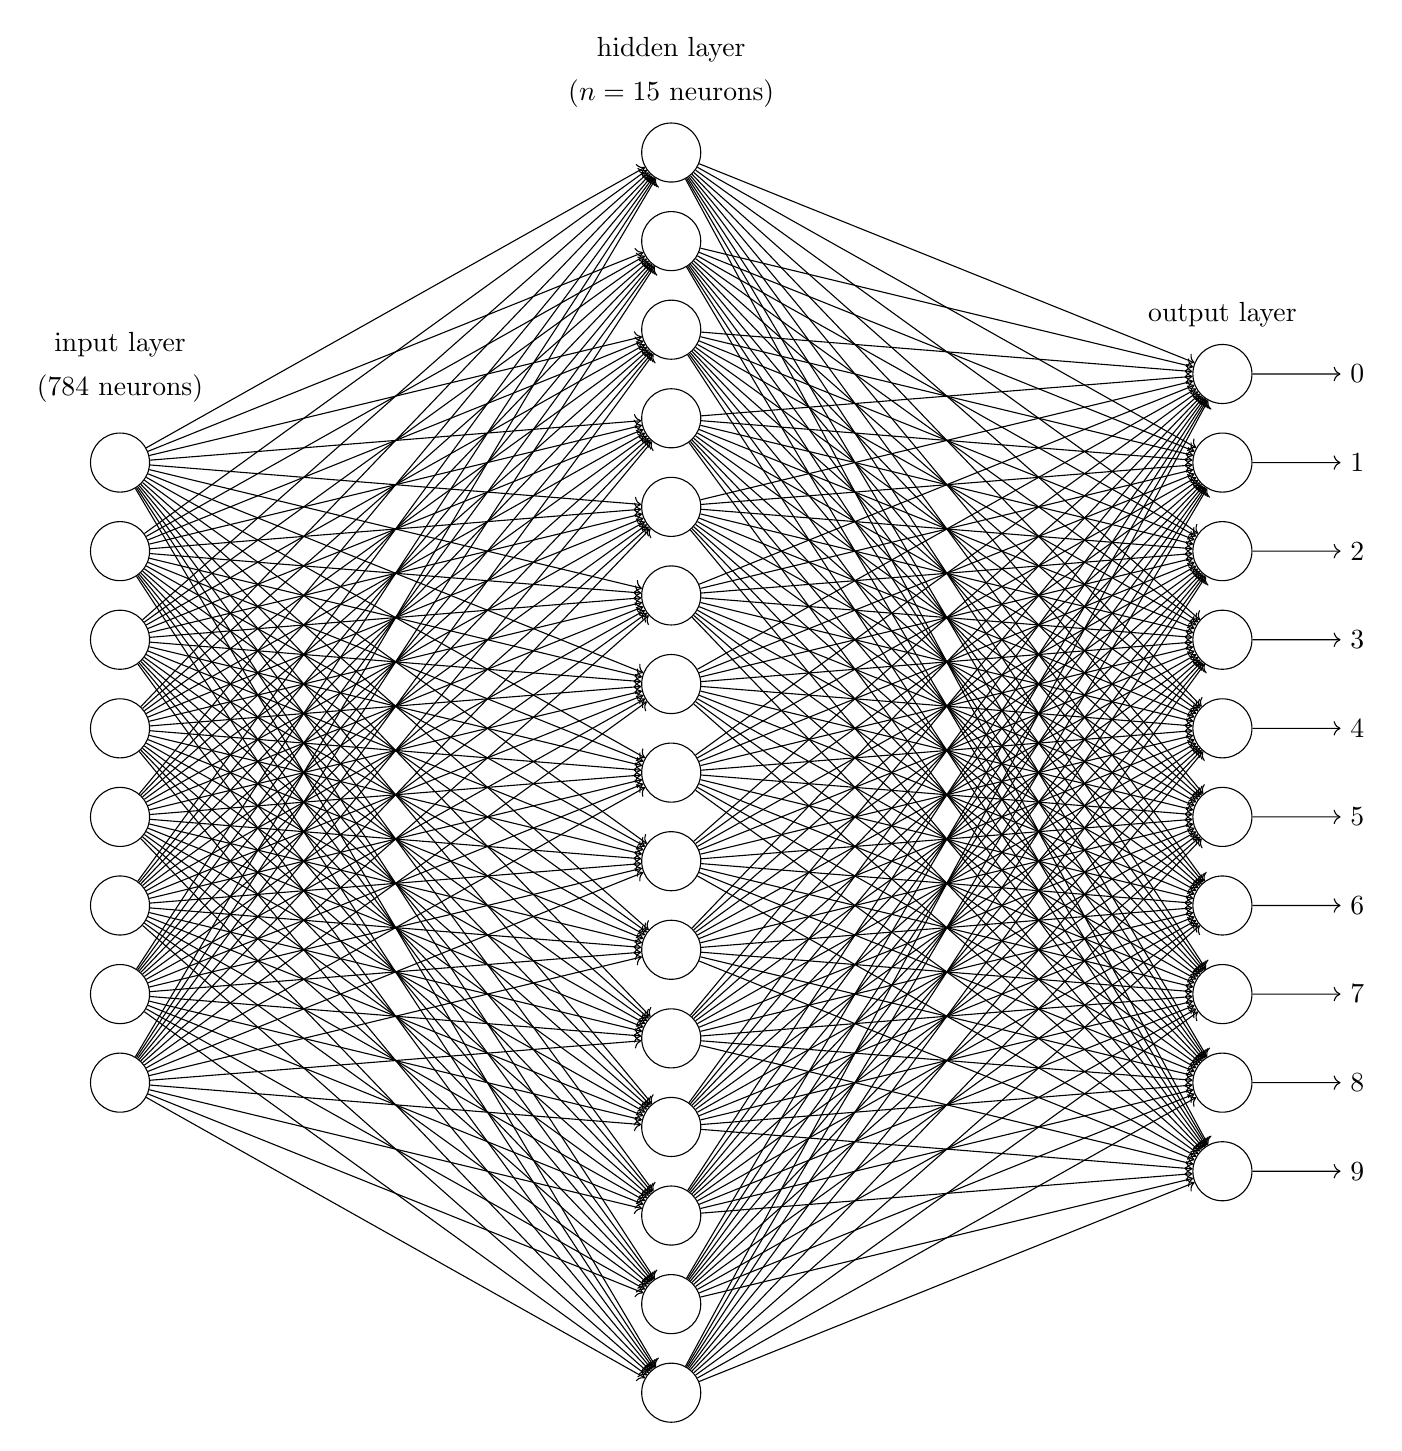
\begin{tikzpicture}[yscale = 0.75]
		\foreach \x in {1, ..., 8}
			\node[circle, draw, minimum size = 0.75cm] (n1\x) at (0, 1.5*\x - 5.25) {};
		\foreach \x in {1, ..., 15}
			\node[circle, draw, minimum size = 0.75cm] (n2\x) at (7, 1.5*\x - 10.5) {};
		\foreach \x in {0, ..., 9}
			\node[circle, draw, minimum size = 0.75cm] (n3\x) at (14, 8.25 - 1.5*\x) {};
		\foreach \x in {1, ..., 8}
			\foreach \y in {1, ..., 15}
				\draw[->] (n1\x) to (n2\y);
		\foreach \x in {1, ..., 15}
			\foreach \y in {0, ..., 9}
				\draw[->] (n2\x) to (n3\y);
		\foreach \x in {0, ..., 9}
			\draw[->] to (n3\x) to (15.5, 8.25 - 1.5*\x) node[right] {\x};
		\node at (0, 8.75) {input layer};
		\node at (0, 8) {(784 neurons)};
		\node at (7, 13.75) {hidden layer};
		\node at (7, 13) {(\(n = 15\) neurons)};
		\node at (14, 9.25) {output layer};
	\end{tikzpicture}	
\end{document}